%=========================================================================
% (c) Michal Bidlo, Bohuslav Křena, 2008


\chapter{Úvod}

\chapter{Digitální forenzní data}
\section{Formáty digitálních forenzních dat}
\section{Způsob uložení}
\section{Existující systémy}

\chapter{Úložiště pro rozsáhlá strukturovaná i nestrukturovaná data}
V této kapitole budou vysvětleny termíny Big data, distribuované databáze a NoSQL databáze, včetně jejich vlastností, výhod a nevýhod.

\section{Big data}
Definicí pro frázi Big data existuje několik. Jedná se o termín použitý na soubory dat, které jsou příliš komplexní z hlediska velikosti a různorodosti, a které je nemožné zpracovávat běžně používanými přístupy a softwarovými nástroji v rozumném čase.

Objem takových dat rychle roste. Vyskytují se v mnoha odvětvích, například sběr informací o počasí, sociální sítě, energetické a telekomunikační společnosti, ekonomie a finančnictví, či data z kamer, měření z různých senzorů apod. Z toho plyne, že se jedná o data různorodých typů, mohou být strukturovaná i nestrukturovaná. Proto je potřeba existence různých technologií pro jejich uložení, zpracování i zobrazení.

\begin{figure}[!h]
  \centering
  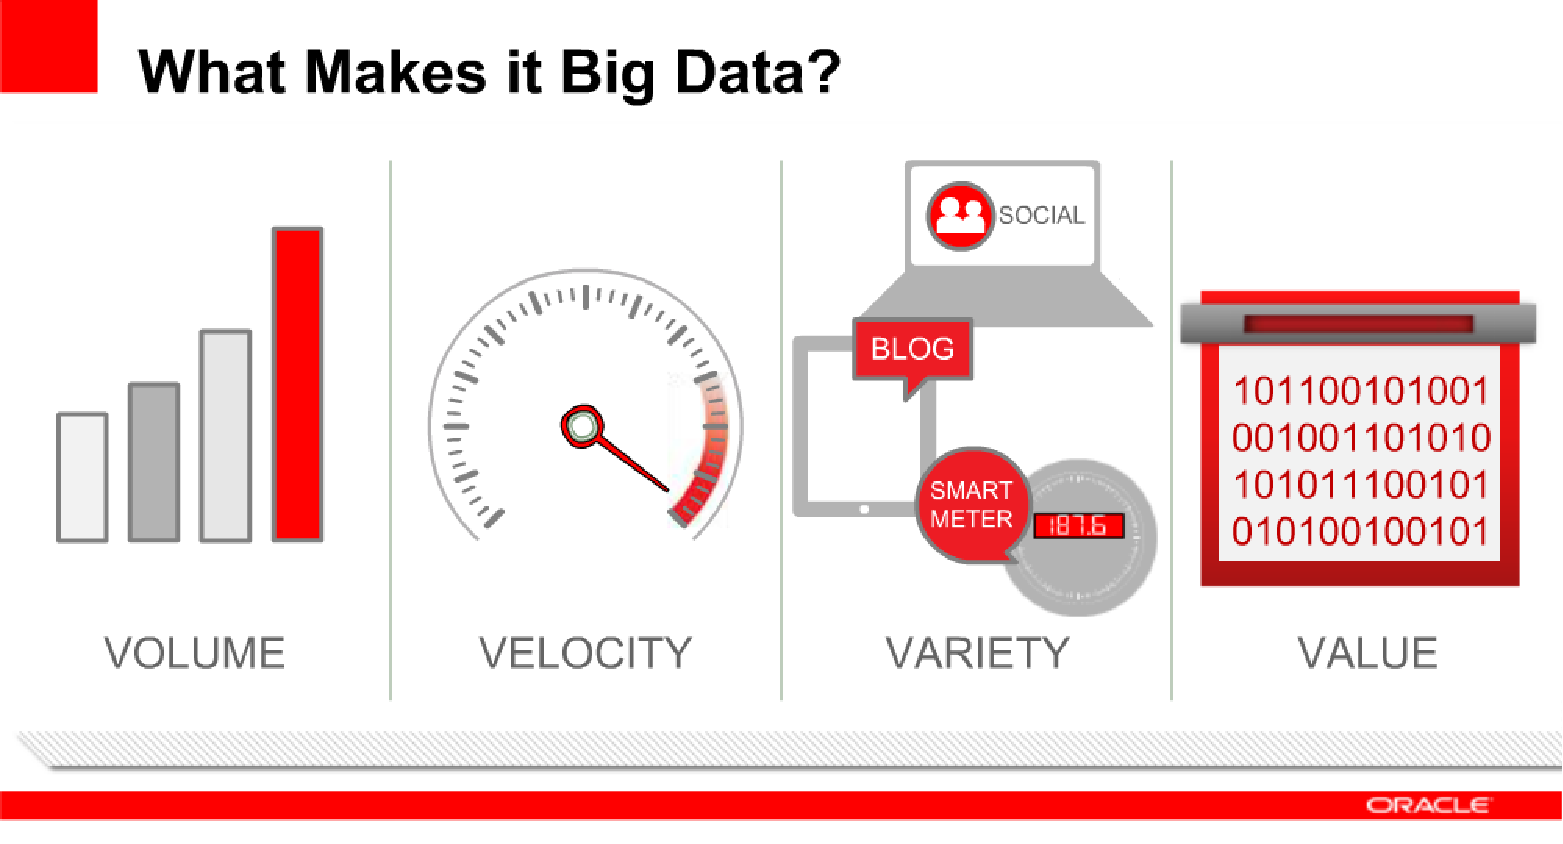
\includegraphics[width=12.5cm]{template-fig/what_makes_data_big_data.pdf}
  \caption{Definice Big data podle Oracle. \cite{johanBigData}}
  \label{FIG_BigData}
\end{figure}

\noindent Big data je často definováno jako 4V z anglických slov Volume, Velocity, Variety a Value. \cite{oracleBigData}

\begin{itemize}
\item Volume – značí množství nebo velikost dat. Big data vyžaduje zpracování vysokých objemů dat neznámých hodnot, například síťový provoz, data sesbírána ze senzorů apod.

\item Velocity – vyjadřuje rychlost z hlediska vzniku dat a potřeby jejich analýzy, některá vyžadují zpracování v reálném čase. Nejdůležitější data se zapisují přímo do paměti, a ne na disk, z důvodu co nejrychlejšího zpracování.

\item Variety – znamená různorodost typů. Jedná se především o nestrukturovaná data, například text, audio, video, data o geografické poloze a další. Jsou na ně kladeny velmi podobné požadavky jako na data strukturovaná – sumarizace, monitorování, důvěrnost. \cite{oracleBigData}

\item Value – data mají vlastní hodnotu, která musí být analyzována a zjištěna. Nejedná se o jednoduchý proces, je stále potřeba nových metod a technik zpracování.
\end{itemize}

\begin{figure}[!h]
  \centering
  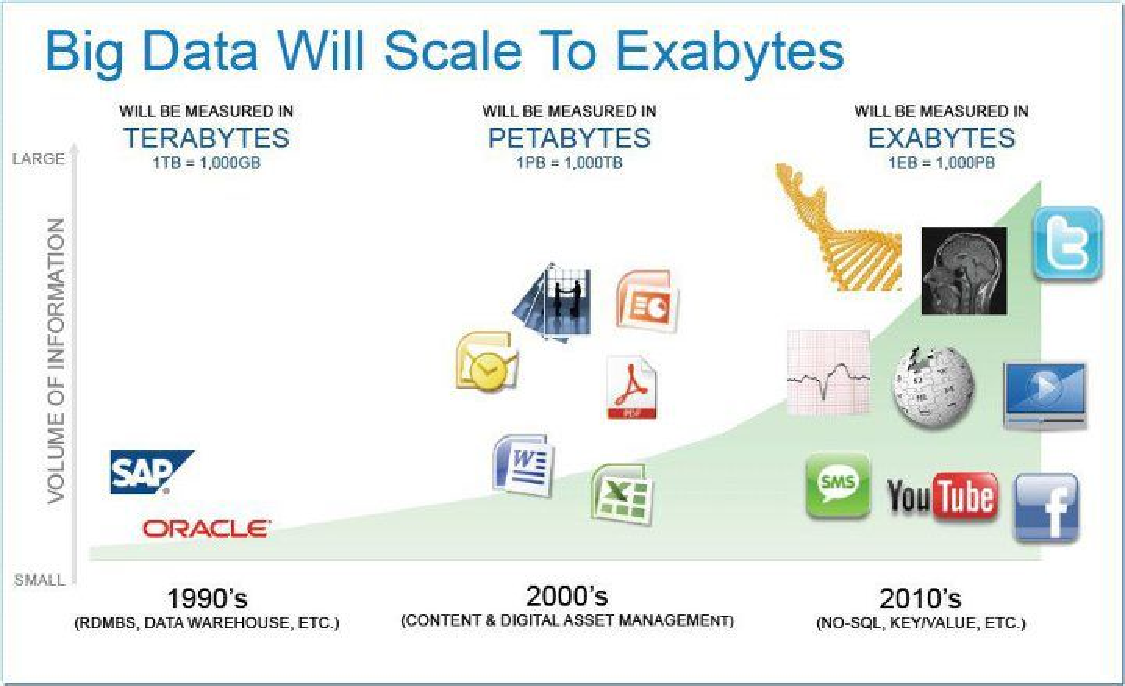
\includegraphics[width=15cm]{template-fig/big_data_exabytes.pdf}
  \caption{S novými technologiemi se masivně zvyšuje růst dat a přibývají nové typy. \cite{rajeshBigData}}
  \label{FIG_BigDataExabytes}
\end{figure}

\noindent Tato práce se zabývá Big daty hlavně typu – PCAP soubory, logy ze síťových zařízení a komunikací. Možnosti uložení Big data budou popsány v následujících podkapitolách.

\section{Distribuované databáze}
Distribuovaná databáze se skládá z většího počtu samostatných databází, které mohou být geograficky rozmístěny na jiných pozicích. Jednotlivé uzly spolu komunikují přes počítačovou síť. Každý uzel je sám o sobě databázový systém. DSŘBD neboli systém řízení distribuované báze dat (anglicky Distributed Database Database Management System) zajišťuje, že se distribuovaná databáze uživatelům jeví jako jedna jediná databáze. Data jsou fyzicky uložena na různých pozicích. Mohou být spravována rozdílnými SŘBD nezávisle na ostatních pozicích. \cite{distributedDBMS}

Systém řízení distribuované báze dat je centralizovaný systém s těmito vlastnostmi 
\cite{distributedDBMS}:

\begin{itemize}
\item Umí vytvářet, získávat, upravovat a mazat distribuované databáze. Zajišťuje důvěrnost a integritu databází.

\item Periodicky synchronizuje databázi a poskytuje mechanismy přístupu tak, aby se databáze uživatelům jevila transparentní.

\item Zajišťuje, že změna dat v kterémkoliv uzlu se promítne i v ostatních uzlech.

\item Je využíván v aplikacích, kde se předpokládá zpracování velkých objemů dat, ke kterým přistupuje současně mnoho uživatelů.
\end{itemize}

\begin{figure}[!h]
  \centering
  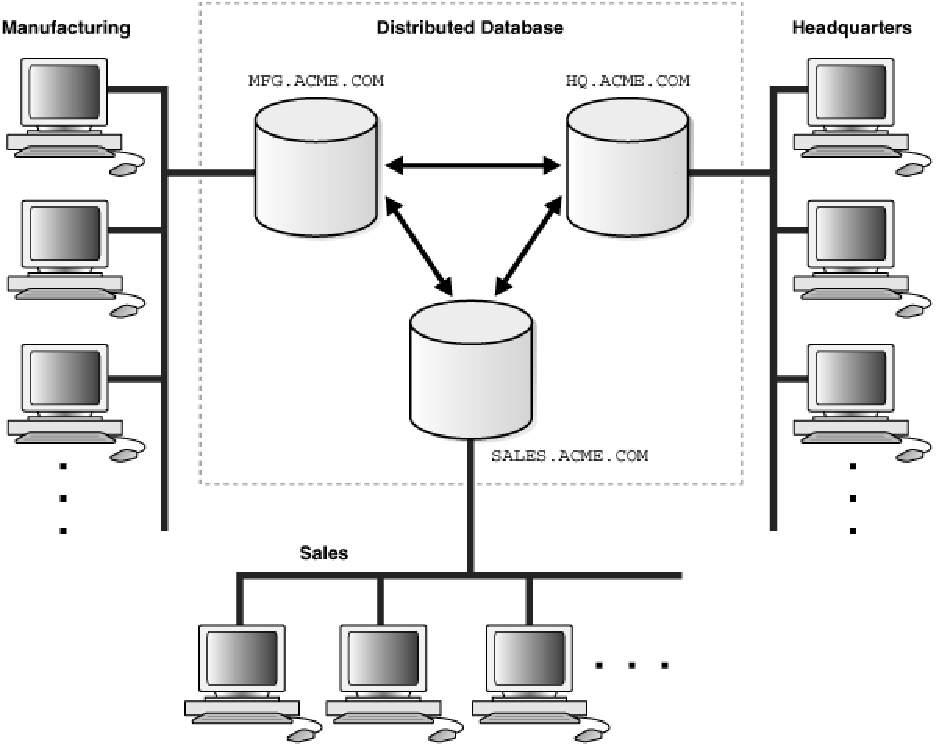
\includegraphics[width=15cm]{template-fig/Distributed_database.pdf}
  \caption{Schéma distribuované databáze a současný přístup více zařízení k ní. \cite{distributedDBMSPic}}
  \label{FIG_DistrDB}
\end{figure}

Výhody
\begin{itemize}
\item Rozšiřitelnost – pokud je potřeba databázový systém rozšířit do nových míst nebo přidat další uzly, stačí přidat nový(é) počítač(e) a lokální data v nové pozici, a nakonec je připojit k distribuovanému systému, bez jakéhokoliv přerušení funkcionality. Podobný postup je při odebrání uzlu.

\item Spolehlivost – když nějaký z připojených uzlů selže, nepřestane distribuovaná databáze fungovat, sníží se maximálně výkon.

\item Ochrana (záloha) dat – při zničení jednoho uzlu a smazání dat z něj, mohou být stejná data zálohována i na jiných uzlech.

\item Výkonnost – pokud jsou data efektivně distribuována, může být uživatelův požadavek uspokojen rychleji. Transakce mohou být také distribuované a provedeny rychleji. 
\end{itemize}

Nevýhody
\begin{itemize}
\item Integrita dat – data musí být průběžně synchronizována na více uzlech, aby na stejné dotazy nebyly z různých uzlů vraceny rozdílné odpovědi.

\item Komunikační režie – i zdánlivě jednoduchá operace může vyžadovat spoustu zbytečné komunikace.

\item Cena – DSŘDB vyžaduje drahý a složitý software ke koordinaci uzlu a zajištění transparentnosti. \cite{distributedDBMS}

\item Mezi další patří – složitost, zabezpečení, řízení souběžného přístupu k datům.
\end{itemize}

\begin{figure}[!h]
  \centering
  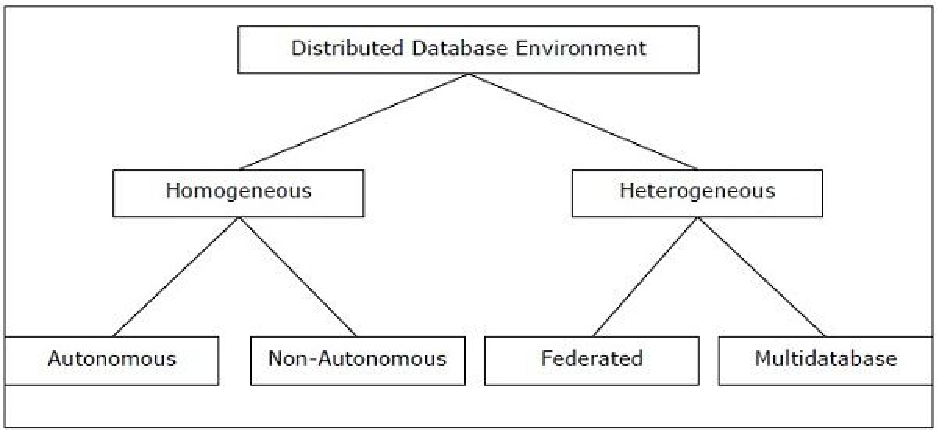
\includegraphics[width=15cm]{template-fig/distributed_database_environments.pdf}
  \caption{Distribuované databáze můžeme rozdělit na homogenní a heterogenní, a tyto ještě dále dělit. \cite{distributedDBMS}}
  \label{FIG_DivDistrDB}
\end{figure}

\noindent Homogenní – všechny uzly používají identické SŘBD a operační systémy. Uzly mají informace o ostatních uzlech a spolupracují při zpracování uživatelských požadavků. Homogenní distribuovaná databáze se navenek jeví uživateli jako jeden systém. Je jednodušší jej navrhnout a spravovat.

Heterogenní – uzly mohou mít rozdílné operační systémy a SŘBD, které nejsou kompatibilní. Mohou také využívat rozdílná schémata (relační, objektově orientované, hierarchické, \ldots). Rozdílnost schématu je hlavním problémem při zpracování dotazu a transakcí. Kvůli tomu je také složité dotazování. \cite{wikiDBMS}

Architekturami distribuovaných databází jsou centrální architektura, klient-server, peer-to-peer, multi-databázová architektura.


\section{NoSQL, disky, úložiště}

\chapter{Návrh distribuovaného úložiště}
\section{Přístup k datům}
\subsection{Sekvenční, náhodný}
\subsection{Dotazování}
\subsection{Big data přístupy}
\section{Architektura}
\section{Aplikační rozhraní}
\section{Technologie}
\subsection{Docker}
\subsection{HDFS, Hadoop, Spark}
\subsection{Cassandra / MongoDB}
\subsection{Zookeeper}
\subsection{MQ broker}

\chapter{Implementace}
\section{Rozšiřitelnost, znuvupoužitelnost}

\chapter{Testování}
\section{Výkon}

\chapter{Závěr}

%=========================================================================
